\documentclass[11pt,a4paper]{article}

\usepackage[utf8]{inputenc}
\usepackage[T1]{fontenc}
\usepackage[brazilian]{babel}
\usepackage[margin=2.2cm]{geometry}
\usepackage{amsmath}
\usepackage{booktabs}
\usepackage{graphicx}
\usepackage{xcolor}
\usepackage{enumitem}
\usepackage[hidelinks]{hyperref}

\setlist{itemsep=2pt, topsep=4pt}

\title{O impacto da representação dos dados no desempenho de classificadores:
um estudo com a base \emph{Dry Bean}}
\author{Arthur Andrade, Fernanda Cruz, Isabelle Gonçalves, Thiago Fraga, Wagner Duarte\\
Introdução ao Reconhecimento de Padrões --- UFMG}
\date{Novembro de 2026}

\begin{document}
\maketitle

%% ====================================================================
\section{Introdução}

A base \emph{Dry Bean} \cite{koklu2020} reúne 13.611 grãos de feijão
de sete variedades (Barbunya, Bombay, Cali, Dermason, Horoz, Seker e Sira),
fotografados e processados por visão computacional. Cada grão é descrito por
16 atributos numéricos de tamanho e forma extraídos da imagem (como área,
perímetro, eixos maior e menor, excentricidade e fatores de forma), sem valores
faltantes. As classes são desbalanceadas: Dermason (26,05\%), Sira (19,37\%),
Seker (14,89\%), Horoz (14,17\%), Cali (11,98\%), Barbunya (9,71\%) e Bombay (3,84\%),
o que motivou o uso do F1-macro como métrica principal.

Escolhemos esta base por reunir propriedades úteis para estudar representação
de dados: os atributos têm escalas muito distintas, há forte
correlação entre vários deles
e o número de amostras permite repetir os
experimentos com validação cruzada. O objetivo não é identificar o classificador
com maior acurácia, mas entender como mudanças na representação dos dados
alteram o comportamento do KNN, do Naive Bayes e do SVM.

Para atender ao enunciado, comparamos os três classificadores exigidos sob
três das cinco estratégias de representação propostas: \emph{normalização/padronização}
(H1), \emph{remoção de atributos redundantes} (H2) e \emph{PCA} (H3).
Seleção de características e geração de novas características não foram utilizadas.

Formulamos três hipóteses, cada uma apoiada em uma propriedade conhecida dos
classificadores:

\begin{itemize}
  \item[H1.] A padronização ajuda muito o KNN e o SVM, mas quase não
  muda o Naive Bayes. \emph{Mecanismo esperado:} KNN e SVM dependem de distâncias e
  são dominados pelos atributos de maior escala; o Naive Bayes modela cada atributo
  separadamente. \emph{Seria refutada se} o ganho do Naive Bayes fosse comparável ao
  dos demais.
  \item[H2.] Remover atributos redundantes ajuda o
  Naive Bayes, mas quase não muda o KNN e o SVM. \emph{Mecanismo esperado:} atributos
  correlacionados violam a independência assumida pelo Naive Bayes, ao passo que KNN
  e SVM lidam melhor com redundância. \emph{Seria refutada se} a remoção
  não melhorasse o Naive Bayes ou alterasse também o KNN e o SVM.
  \item[H3.] Com o mesmo número de dimensões, o PCA mantém um desempenho
  melhor do que a remoção de atributos correlacionados. \emph{Mecanismo esperado:}
  o PCA combina todos os atributos e preserva a variância, enquanto a remoção
  descarta atributos inteiros. \emph{Seria refutada se} a remoção igualasse ou
  superasse o PCA para o mesmo número de dimensões.
\end{itemize}

%% ====================================================================
\section{Metodologia}

\paragraph{Classificadores.}
Foram utilizados o KNN, o Naive Bayes gaussiano e o SVM com núcleo RBF, todos da
biblioteca \texttt{scikit-learn} e com hiperparâmetros padrão
(KNN com $k=5$; SVM com $C=1$ e $\gamma$ ``\texttt{scale}''). Não houve ajuste de
hiperparâmetros, o que é uma limitação discutida na Seção~\ref{sec:concl}.

\paragraph{Representações dos dados.}
\begin{itemize}
  \item H1 (escala): dados brutos, normalização Min--Max e
  padronização (\emph{z-score}).
  \item H2 (redundância): remoção de atributos por correlação de
  Pearson, com limiares $|r| > 0{,}99$, $0{,}95$ e $0{,}90$, além da base completa
  como referência.
  \item H3 (PCA $\times$ remoção): PCA com o mesmo número de
  dimensões que restou em cada limiar de remoção da H2, para comparar as duas
  estratégias em igualdade de dimensão.
\end{itemize}

\paragraph{Protocolo experimental.}
Utilizamos validação cruzada estratificada com 5 \emph{folds} e 3 repetições
(15 execuções por configuração), com \texttt{random\_state}$=42$.
Todas as transformações (escala, seleção e PCA) são ajustadas
apenas nos dados de treino de cada \emph{fold}, dentro de um
\texttt{Pipeline}, para evitar vazamento de informação.

\paragraph{Métricas.}
A métrica principal é o F1-macro, escolhida por causa do desbalanceamento
entre as classes. Também reportamos a acurácia, o tempo de treino e predição e
matrizes de confusão agregadas. Os resultados são apresentados como média
$\pm$ desvio padrão das 15 execuções.

%% ====================================================================
\section{Resultados e Discussão}
% Pessoas 1, 2, 3 (cada uma ~1/2 página) e Pessoa 5 (comparação geral).

\subsection{Impacto da escala dos atributos (H1)}

A Tabela~\ref{tab:resultados_h1} resume o F1-macro (média $\pm$ desvio padrão nas 15 execuções) e o tempo médio de treino e predição sob dados brutos, 
normalização Min-Max e padronização (\textit{z-score}).

\begin{table}[htbp]
    \centering
    \caption{F1-macro ($\pm$ DP) e tempo médio de execução nas três representações da H1.}
    \label{tab:resultados_h1}
    \footnotesize
    \setlength{\tabcolsep}{4pt}
    \begin{tabular}{lccccc}
        \toprule
        \textbf{Classificador} & \textbf{Brutos} & \textbf{Min-Max} & \textbf{Padronizados} & \textbf{Ganho (\textit{z})} & \textbf{\shortstack{Tempo \\ (bruto $\rightarrow$ \textit{z})}} \\
        \midrule
        KNN & 72,70\% $\pm$ 0,91\% & 93,24\% $\pm$ 0,46\% & 93,51\% $\pm$ 0,56\% & +20,81 p.p. & 0,051s $\rightarrow$ 0,046s \\
        SVM (RBF) & 59,62\% $\pm$ 0,74\% & 93,61\% $\pm$ 0,47\% & 94,02\% $\pm$ 0,49\% & +34,39 p.p. & 2,155s $\rightarrow$ 0,599s \\
        Naive Bayes (padrão) & 76,50\% $\pm$ 0,89\% & 90,63\% $\pm$ 0,56\% & 90,63\% $\pm$ 0,56\% & +14,13 p.p. & 0,011s $\rightarrow$ 0,019s \\
        Naive Bayes \\(\texttt{var\_smoothing=0}) & 90,63\% $\pm$ 0,56\% & 90,63\% $\pm$ 0,56\% & 90,63\% $\pm$ 0,56\% & 0,00 p.p. & 0,010s $\rightarrow$ 0,017s \\
        \bottomrule
    \end{tabular}
\end{table}

% \begin{figure}[htbp]
%     \centering
%     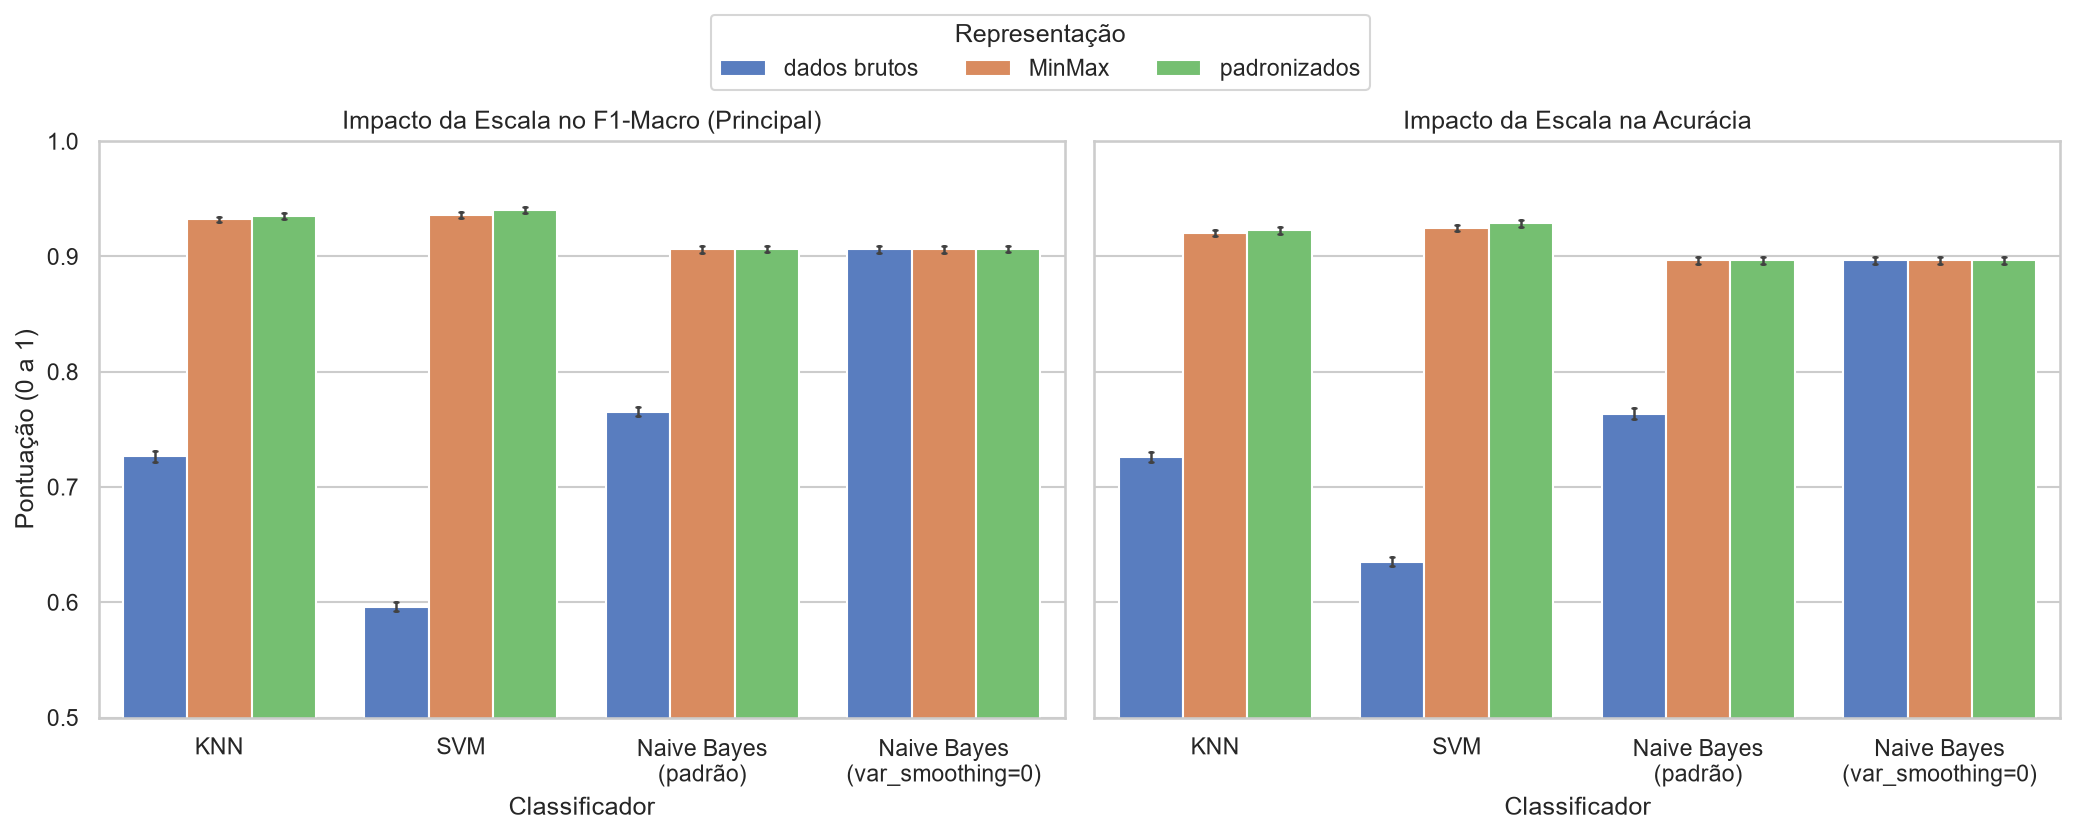
\includegraphics[width=\textwidth]{resultados/H1/h1_comparacao_metricas.png}
%     \caption{F1-macro e acurácia (média $\pm$ DP) nas três representações da H1.}
%     \label{fig:h1}
% \end{figure}

\textbf{KNN e SVM.} Nos dados brutos, atributos de grande escala (\texttt{Area}, \texttt{ConvexArea}) dominam as distâncias e anulam variáveis decimais 
(\texttt{ShapeFactor}). Com a padronização (\textit{z-score}, ligeiramente superior ao Min-Max), o SVM foi do pior ao melhor desempenho ($+34{,}39$~p.p. 
e $3{,}6\times$ mais rápido), recuperando Barbunya ($6{,}2\% \rightarrow 90{,}4\%$) e Seker ($26{,}4\% \rightarrow 94{,}9\%$); o KNN ganhou $+20{,}81$~p.p. 
com menor variância entre \textit{folds}.

\textbf{Naive Bayes e avaliação da H1.} O ganho de $+14{,}13$~p.p. na configuração padrão do \texttt{scikit-learn} decorre de um artefato numérico do 
\texttt{var\_smoothing=1e-9}, que soma $10^{-9}$ da maior variância (\texttt{Area}, $\sim 10^8$) a todos os atributos, distorcendo variáveis decimais. 
Com \texttt{var\_smoothing=0}, o desempenho é idêntico nas três escalas ($90{,}63\% \pm 0{,}56\%$). A H1 é confirmada teoricamente, embora a padronização 
siga recomendável na prática para neutralizar esse viés em bases com variâncias heterogêneas.

\subsection{Remoção de atributos redundantes (H2)}
% Pessoa 2. Inserir a figura da H2 como nas outras seções, por exemplo:
% \begin{figure}[htbp]
%     \centering
%     \includegraphics[width=\textwidth]{resultados/H2/NOME_DA_FIGURA.png}
%     \caption{...}
%     \label{fig:h2}
% \end{figure}

\subsection{PCA $\times$ remoção de atributos com a mesma dimensão (H3)}
% Pessoa 3. Figura já inserida; escrever a análise abaixo dela.

\begin{figure}[htbp]
    \centering
    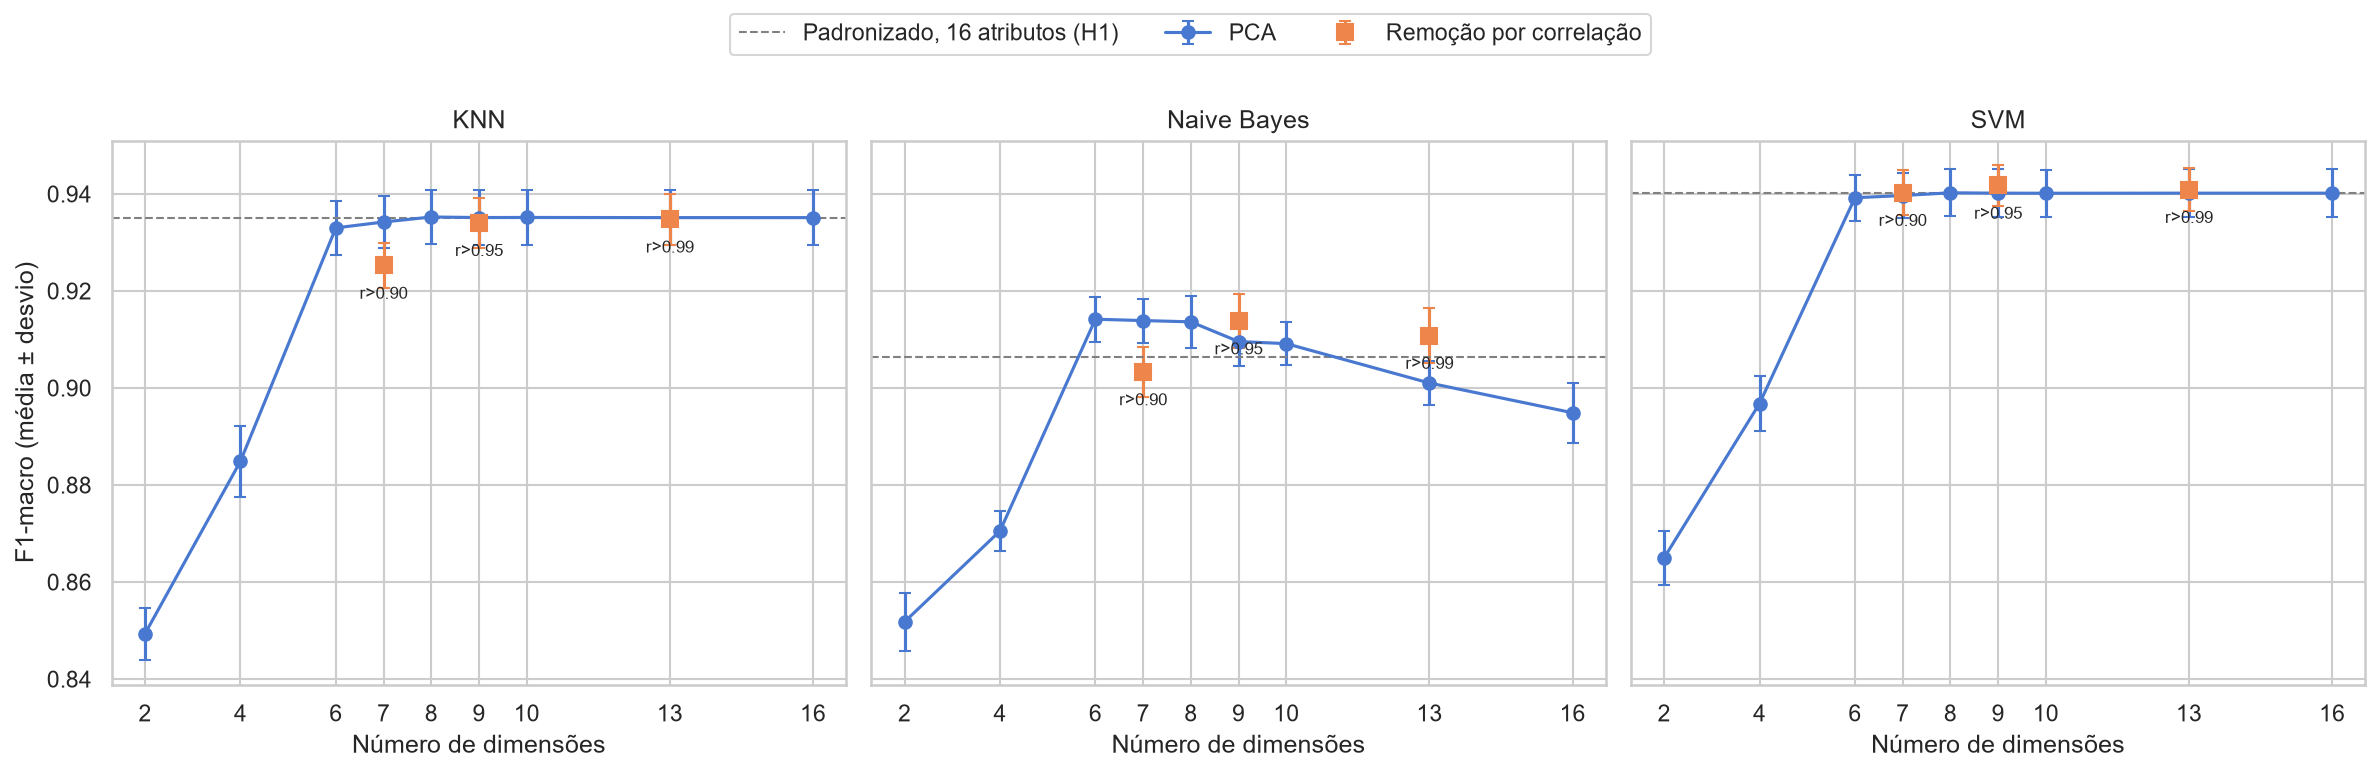
\includegraphics[width=\textwidth]{resultados/H3/h3_f1_por_dimensao.png}
    \caption{F1-macro em função do número de dimensões: PCA (linha) e remoção por
    correlação (quadrados). A linha tracejada indica os 16 atributos padronizados.}
    \label{fig:h3}
\end{figure}

%% ---------------------------------------------------------------------
\subsection{Comparação geral}\label{sec:geral}
% Pessoa 5. Tabela gerada por codigos/comparacao_geral.py
% (rodar de novo quando a H2 existir: a coluna "Melhor H2" entra sozinha).

\begin{table}[htbp]
    \centering
    \caption{F1-macro (\%) nos dados brutos e na melhor representação de cada hipótese (entre parênteses, ganho em p.p.\ sobre os dados brutos).}
    \label{tab:comparacao_geral}
    \footnotesize
    \begin{tabular}{lccc}
        \toprule
        \textbf{Classificador} & \textbf{Brutos} & \textbf{Melhor H1} & \textbf{Melhor H3} \\
        \midrule
        KNN & 72,70 & \shortstack{93,51 (+20,81)\\\scriptsize padronizados} & \shortstack{93,52 (+20,82)\\\scriptsize PCA k=8} \\
        Naive Bayes & 76,50 & \shortstack{90,63 (+14,13)\\\scriptsize MinMax} & \shortstack{91,42 (+14,91)\\\scriptsize PCA k=6} \\
        SVM & 59,62 & \shortstack{94,02 (+34,39)\\\scriptsize padronizados} & \shortstack{94,17 (+34,55)\\\scriptsize remocao r$>$0.95} \\
        \bottomrule
    \end{tabular}
\end{table}


A Tabela~\ref{tab:comparacao_geral} reúne, para cada classificador, os dados brutos,
os dados padronizados e a melhor representação obtida nas demais hipóteses. Como os
\emph{pipelines} da H2 e da H3 padronizam os dados antes da remoção ou do PCA, o efeito
próprio dessas técnicas é medido em relação aos dados padronizados, e não aos brutos.

O quadro revela uma hierarquia clara. A escala dos atributos é, de longe, o fator
dominante: a padronização eleva o F1-macro em 14 a 34~p.p. Uma vez padronizados os
dados, a redução de dimensionalidade altera o desempenho em menos de 1~p.p. O Naive
Bayes é o único com ganho perceptível (+0,78~p.p.\ com PCA de 6 componentes), o que é
coerente com a violação da independência condicional pelos atributos correlacionados;
para o KNN e o SVM, as diferenças ($\leq$0,16~p.p.) são menores que um desvio padrão
entre \emph{folds}. Por outro lado, a base admite forte compressão: com apenas 6
componentes principais, nenhum classificador perde mais de 0,25~p.p.\ em relação
aos 16 atributos padronizados.
\textcolor{red}{[Completar com a H2 quando os resultados estiverem prontos.]}

Por fim, a representação pesou mais do que a escolha do classificador: nos dados brutos,
o F1-macro varia de 59,6\% (SVM) a 76,5\% (Naive Bayes), uma diferença de 17~p.p.\ e com
o SVM em último lugar; após a padronização, os três ficam a menos de 3,5~p.p.\ entre si
e o SVM passa ao primeiro lugar.

%% ====================================================================
\section{Conclusão}\label{sec:concl}
% Pessoa 5.

Este trabalho investigou como a representação dos dados afeta o KNN, o Naive Bayes e o
SVM na base \emph{Dry Bean}. As hipóteses foram avaliadas da seguinte forma:

\begin{itemize}
  \item \textbf{H1 (confirmada):} a padronização foi decisiva para o KNN
  (+20,8~p.p.) e o SVM (+34,4~p.p.). O Naive Bayes só variou por um artefato
  numérico do \texttt{var\_smoothing}; sem ele, seu desempenho foi idêntico nas três
  representações.
  \item \textbf{H2:} \textcolor{red}{[completar após os resultados da H2].}
  \item \textbf{H3 (parcialmente confirmada):} o PCA superou a remoção apenas na
  redução mais agressiva (7 dimensões), para o KNN (+0,89~p.p.) e o Naive Bayes
  (+1,06~p.p.), em 15 de 15 \emph{folds} (Wilcoxon, $p<0{,}001$). Com 9 e 13 dimensões,
  a vantagem do PCA no KNN caiu para no máximo 0,11~p.p.\ e se inverteu no Naive Bayes
  (remoção melhor em até 0,98~p.p.); no SVM, as diferenças ficaram abaixo de 0,2~p.p. Ou seja, a vantagem do PCA só aparece quando a remoção precisa descartar
  atributos informativos.
\end{itemize}

A principal descoberta é que, nesta base, o pré-processamento de escala importa mais
do que a escolha do classificador ou a redução de dimensionalidade.

\paragraph{Limitações.}
(i) Todos os classificadores usaram hiperparâmetros padrão; um ajuste de $k$, $C$ e
$\gamma$ poderia alterar a ordem entre eles e a sensibilidade a cada representação.
(ii) Foi usada uma única base, cujos atributos geométricos são fortemente
correlacionados entre si, o que limita a generalização das conclusões.
(iii) A remoção por correlação é gulosa e depende da ordem dos atributos.
(iv) Várias diferenças observadas após a padronização são menores que 1~p.p., da
ordem do desvio padrão entre \emph{folds}, e só a H3 foi acompanhada de teste
estatístico.

%% ====================================================================
\begin{thebibliography}{9}
\bibitem{koklu2020}
M.~Koklu and I.~A. Özkan.
\newblock Multiclass classification of dry beans using computer vision and machine
learning techniques.
\newblock \emph{Computers and Electronics in Agriculture}, 174:105507, 2020.
\end{thebibliography}

\end{document}